%% Beginning of file 'sample631.tex'
%%
%% Modified 2021 March
%%
%% This is a sample manuscript marked up using the
%% AASTeX v6.31 LaTeX 2e macros.
%%
%% AASTeX is now based on Alexey Vikhlinin's emulateapj.cls 
%% (Copyright 2000-2015).  See the classfile for details.

%% AASTeX requires revtex4-1.cls and other external packages such as
%% latexsym, graphicx, amssymb, longtable, and epsf.  Note that as of 
%% Oct 2020, APS now uses revtex4.2e for its journals but remember that 
%% AASTeX v6+ still uses v4.1. All of these external packages should 
%% already be present in the modern TeX distributions but not always.
%% For example, revtex4.1 seems to be missing in the linux version of
%% TexLive 2020. One should be able to get all packages from www.ctan.org.
%% In particular, revtex v4.1 can be found at 
%% https://www.ctan.org/pkg/revtex4-1.

%% The first piece of markup in an AASTeX v6.x document is the \documentclass
%% command. LaTeX will ignore any data that comes before this command. The 
%% documentclass can take an optional argument to modify the output style.
%% The command below calls the preprint style which will produce a tightly 
%% typeset, one-column, single-spaced document.  It is the default and thus
%% does not need to be explicitly stated.
%%
%% using aastex version 6.3
\documentclass[linenumbers]{aastex631}

\newcommand{\vdag}{(v)^\dagger}
\newcommand\aastex{AAS\TeX}
\newcommand\latex{La\TeX}
\newcommand\eppsilon{$\varepsilon$ppsilon\xspace}

\graphicspath{{./}{figures/}}
%% This is the end of the preamble.  Indicate the beginning of the
%% manuscript itself with \begin{document}.

\begin{document}

\title{Investigating a FHD/Eppsilon power spectrum systematic likely caused by snapshot mosaicing}

%% LaTeX will automatically break titles if they run longer than
%% one line. However, you may use \\ to force a line break if
%% you desire. In v6.31 you can include a footnote in the title.

%% A significant change from earlier AASTEX versions is in the structure for 
%% calling author and affiliations. The change was necessary to implement 
%% auto-indexing of affiliations which prior was a manual process that could 
%% easily be tedious in large author manuscripts.
%%
%% The \author command is the same as before except it now takes an optional
%% argument which is the 16 digit ORCID. The syntax is:
%% \author[xxxx-xxxx-xxxx-xxxx]{Author Name}
%%
%% This will hyperlink the author name to the author's ORCID page. Note that
%% during compilation, LaTeX will do some limited checking of the format of
%% the ID to make sure it is valid. If the "orcid-ID.png" image file is 
%% present or in the LaTeX pathway, the OrcID icon will appear next to
%% the authors name.
%%
%% Use \affiliation for affiliation information. The old \affil is now aliased
%% to \affiliation. AASTeX v6.31 will automatically index these in the header.
%% When a duplicate is found its index will be the same as its previous entry.
%%
%% Note that \altaffilmark and \altaffiltext have been removed and thus 
%% can not be used to document secondary affiliations. If they are used latex
%% will issue a specific error message and quit. Please use multiple 
%% \affiliation calls for to document more than one affiliation.
%%
%% The new \altaffiliation can be used to indicate some secondary information
%% such as fellowships. This command produces a non-numeric footnote that is
%% set away from the numeric \affiliation footnotes.  NOTE that if an
%% \altaffiliation command is used it must come BEFORE the \affiliation call,
%% right after the \author command, in order to place the footnotes in
%% the proper location.
%%
%% Use \email to set provide email addresses. Each \email will appear on its
%% own line so you can put multiple email address in one \email call. A new
%% \correspondingauthor command is available in V6.31 to identify the
%% corresponding author of the manuscript. It is the author's responsibility
%% to make sure this name is also in the author list.
%%
%% While authors can be grouped inside the same \author and \affiliation
%% commands it is better to have a single author for each. This allows for
%% one to exploit all the new benefits and should make book-keeping easier.
%%
%% If done correctly the peer review system will be able to
%% automatically put the author and affiliation information from the manuscript
%% and save the corresponding author the trouble of entering it by hand.

%\correspondingauthor{August Muench}
%\email{greg.schwarz@aas.org, gus.muench@aas.org}

\author{Lindsay Berkhout}
\affiliation{Arizona State University \\ School of Earth and Space Exploration}


%% Note that the \and command from previous versions of AASTeX is now
%% depreciated in this version as it is no longer necessary. AASTeX 
%% automatically takes care of all commas and "and"s between authors names.

%% AASTeX 6.31 has the new \collaboration and \nocollaboration commands to
%% provide the collaboration status of a group of authors. These commands 
%% can be used either before or after the list of corresponding authors. The
%% argument for \collaboration is the collaboration identifier. Authors are
%% encouraged to surround collaboration identifiers with ()s. The 
%% \nocollaboration command takes no argument and exists to indicate that
%% the nearby authors are not part of surrounding collaborations.

%% Mark off the abstract in the ``abstract'' environment.

\section{Introduction}
This memo investigates the origins of a systematic in the FHD/\eppsilon{} pipeline which has a potentially large impact on the power spectrum. This systematic was originally identified in a standard run of data through FHD and \eppsilon{} with a single zenith pointing observation from the golden day of the Murchison Widefield Array's 2013 observing season. It was then reconfirmed in simulation, using the same observation as the pointing reference for the simulation. The systematic appears to arise from the portion of the pipeline that integrates snapshots into a single cube or (less likely) in the fourier transform from image to power spectrum. It is strongest when considering single snapshots and decreases when more observations are added. Further progress will require rework of the interpolation code used to grid square images into healpix. \newline 

\section{Description of the steps to produce the issue}
All plots shown in this memo are from simulated visibilities produced using the in-situ simulator provided by FHD. The modified gridding kernel as described in \cite{Barry} is applied to the beam. This requires seperate runs for calibration and the rest of the pipeline, as the modified kernel cannot be used to generate calibration solutions. \newline
The "cause" of the systematic appears to be changing the keyword ps\_kspan. The default value of this keyword is 600 wavelengths, and the limited span is 200 wavelengths. The default span shows the systematic in the model power spectra. This keyword controls the UV plane dimension in wavelengths for Healpix cube generation.  \newline


\section{Description of systematic}
This systematic appears as large excess power above the wedge seen in power spectra of single observations, which we have dubbed The Smudge seen in figures \ref{fig:smudge1}. The smudge amplitude at short baselines increases as longer baselines are included in the healpix mosiac. We do not see this issue when cutting out the longer baselines in our analysis. The "smudge" appears when the cut is left at the default 600 wavelengths. The plots for this memo are showing model 2D power spectra for just the xx pol, however the systematic appears on both pols. 
\\
\begin{figure}[htb]
        \centering
        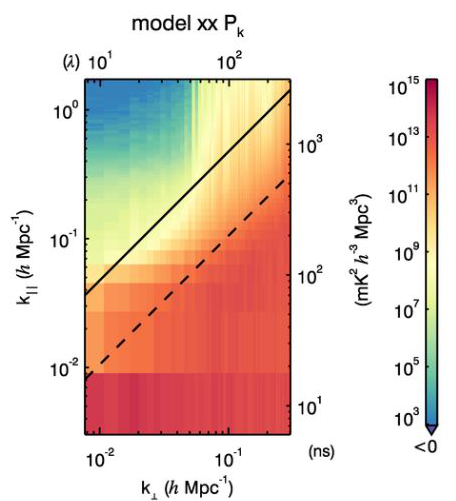
\includegraphics[scale=.5]{default.png}
        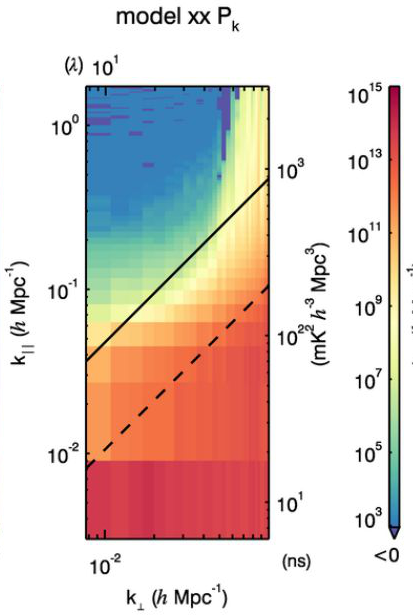
\includegraphics[scale=.4]{limited.png}
        \caption{Left: Simulated 2D power spectrum produced with the default UV plane span of 600 wavelengths. Excess power is seen above the solid black line in the lower left portion. Right: limited UV plane span of 200 wavelengths. Excess power is reduced above the solid black line in the lower left portion.}
        \label{fig:smudge1}
\end{figure}

% \begin{figure}[h!]{0.4\textwidth}
%         \centering
        
%         \caption{Simulated 2D power spectrum produced with the limited UV plane span of 200 wavelengths. Excess power is reduced above the solid black line in the lower left portion.}
%         \label{fig:smudge2}
% \end{figure}

\section{UVF test}
One potential source of error in the imaging process is the re-gridding of snapshots to healpix. This step has the potential to introduce spectral features as the frequency dependent point spread function moves with respect to the fixed sky grid. I set out to isolate the part of the pipeline in which the aliasing occurred by eliminating the Healpix cube creation step. It is possible to create a power spectrum in 
\eppsilon{} with UVF space cubes, rather than Healpix cubes, for a single observation. The fundamental purpose of interpolating to a Healpix grid is to line up a basis for observations in different parts of the sky, which is unnecessary when using only a single observation. 
This pipeline rerouting is shown by the blue arrows in figure \ref{fig:uvfreroute} . 

\begin{figure}[h!]
    \centering
    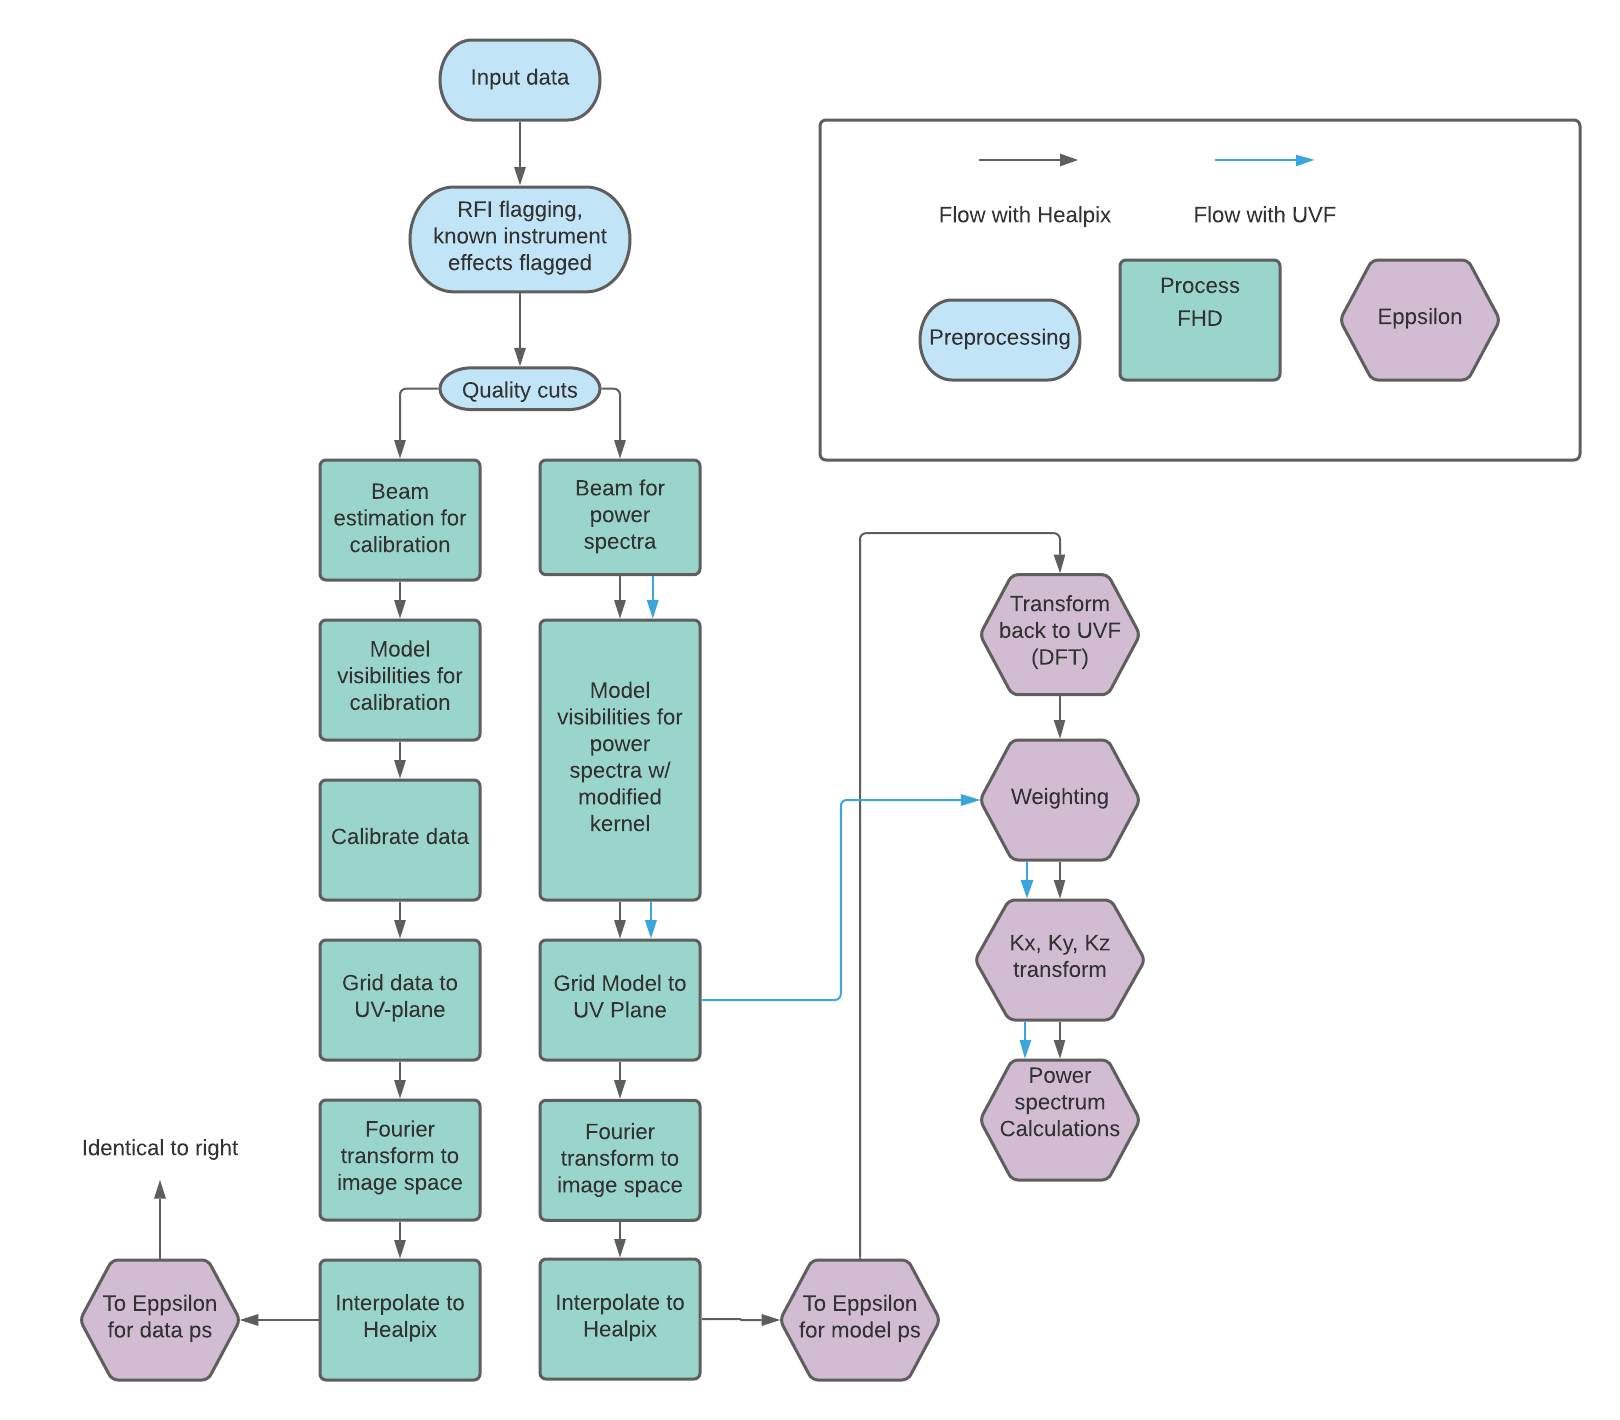
\includegraphics[scale=.4]{uvftest.png}
    \caption{Rerouting of the FHD/\eppsilon{} pipeline done to test the UVF input functionality of Eppsilon. The UVF pipeline flow is indicated by the blue arrows, and the Healpix flow by the black arrows.}
    \label{fig:uvfreroute}
\end{figure}


The UVF cube power spectrum looks remarkably improved from the Healpix interpolated spectrum, with the magnitude of power in the EOR window similar to a Healpix power spectrum calculated with a 200 wavelength uv-plane. The result of this test is shown in figure \ref{fig:uvfresult}. This narrows down the possible sources of aliasing to the interpolation routine or use of Healpix in FHD, or the DFT in \eppsilon{} (or, some combination of these steps). \\
\begin{figure}[!h]
    \centering
    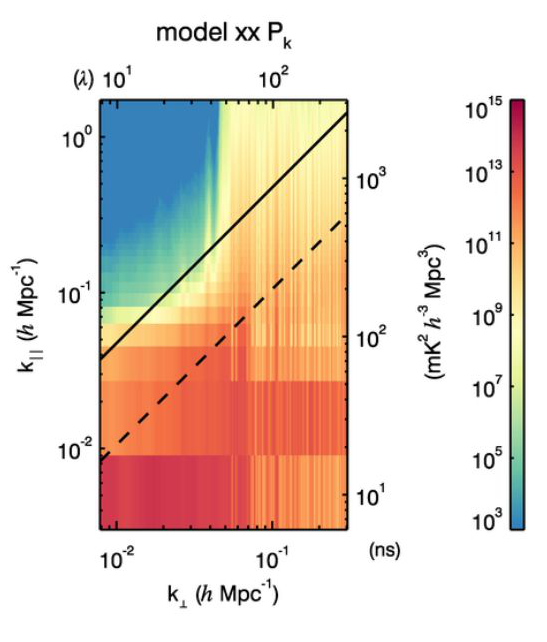
\includegraphics[scale=.4]{uvf.png}
    \caption{2D power spectrum showing results of the UVF input test. Power in the EoR window looks remarkably reduced.}
    \label{fig:uvfresult}
\end{figure}

\section{Orthoslant Interpolation}
The next test further narrowed the cause of aliasing by re-introducing the interpolation, but instead of Healpix, using a rectilinear grid very close to that of the original snapshot. This will also have the effect of allowing \eppsilon{} to use a fast fourier transform (FFT) instead of a DFT. Instead of interpolating to a Healpix map, an orthoslant grid is pulled from a zenith pointing observation. Then, a carefully chosen observation nearby is interpolated to this grid. This observation is chosen such that the interpolation routine will have to do some amount of work to match to the nearby grid, but not so far that the observation is completely mismatched to the grid. The goal is to choose an observation that will result in a similar amount of interpolation as going to a Healpix map. This rerouting of the pipeline is shown in figure \ref{fig:orthoslantflow}. 
\\
\begin{figure}[!h]
    \centering
    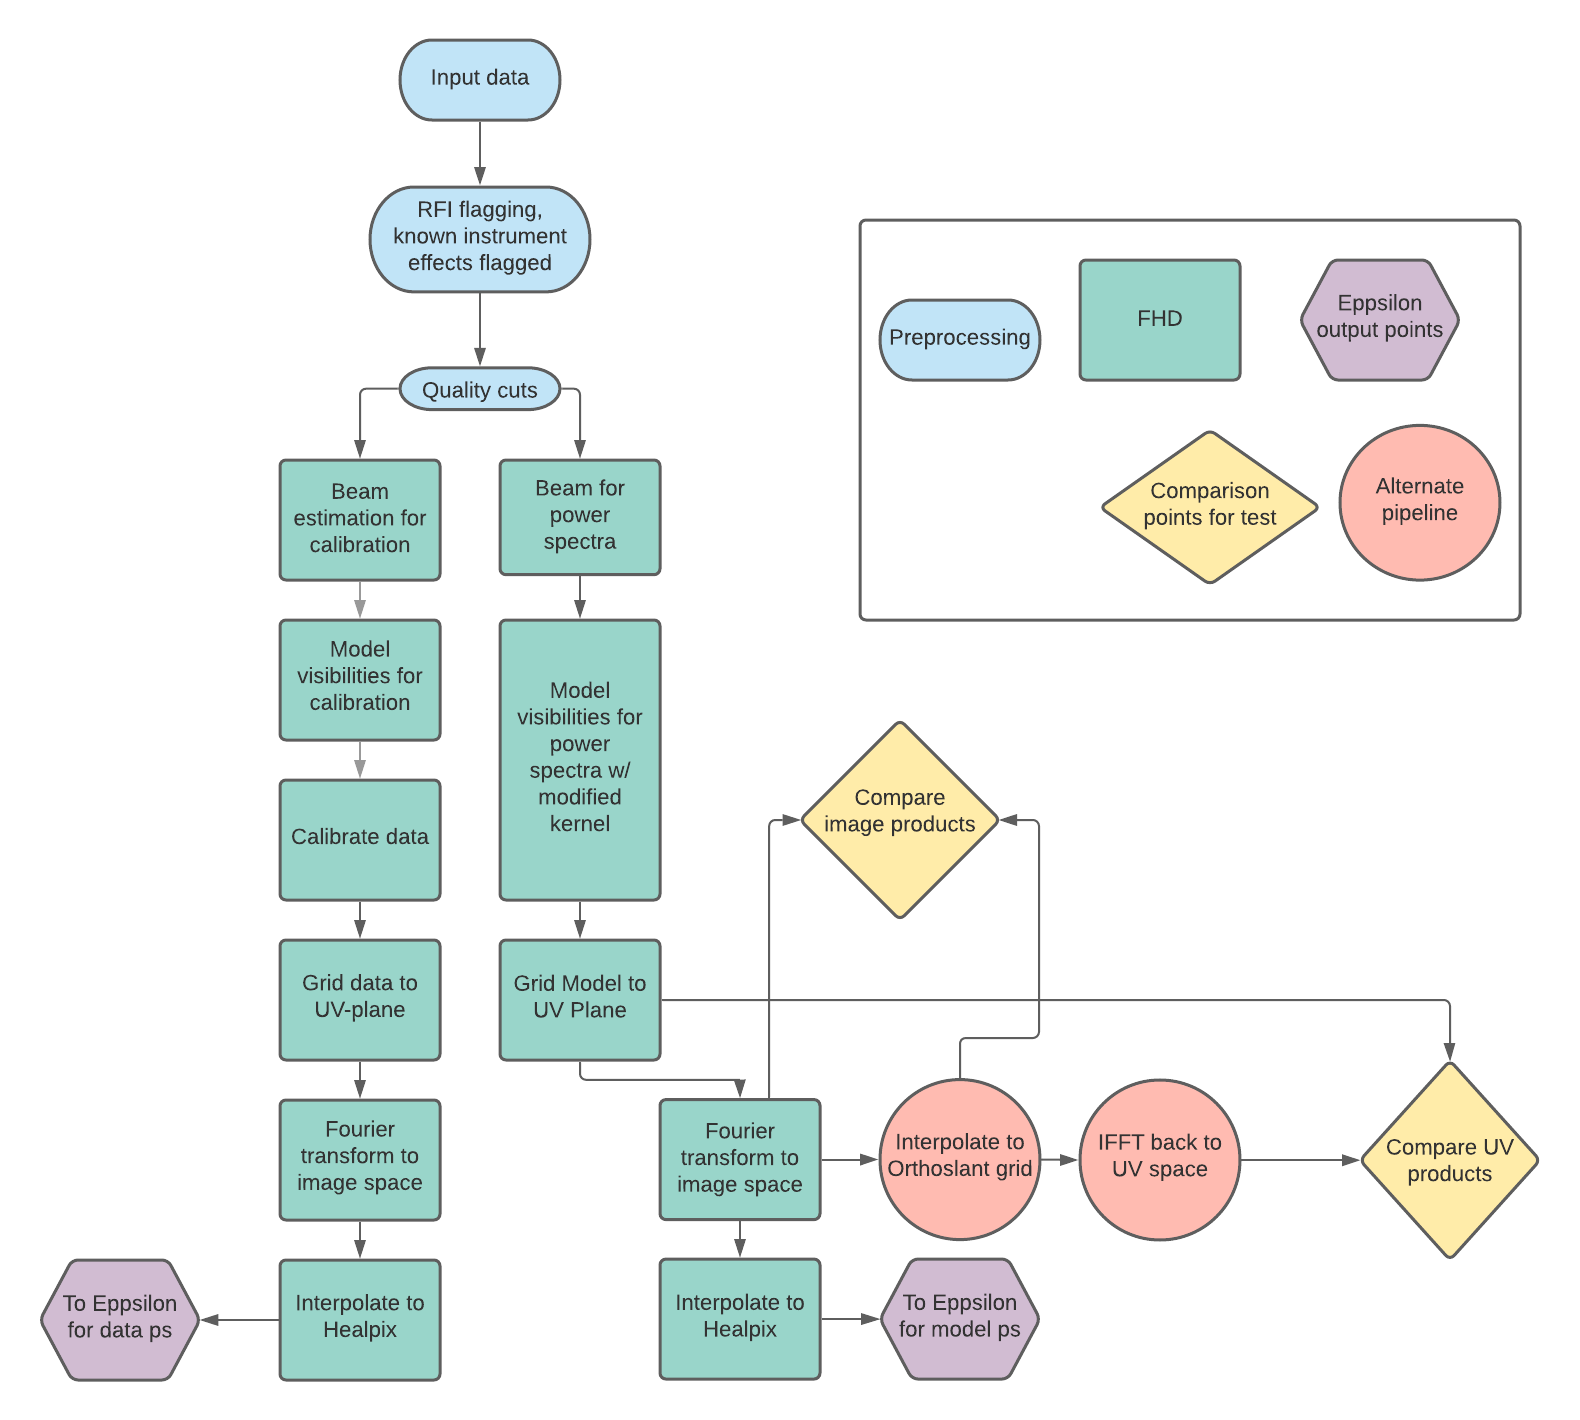
\includegraphics[scale=.2]{FHD pipeline diagram.png}
    \caption{Rerouting of the FHD pipeline to indicate paths for the orthoslant gridding and  Healpix gridding. The alternate pipeline is indicated in pink circles, and the regular pipeline is indicated in green squared. Test output products are indicated in yellow diamonds.}
    \label{fig:orthoslantflow}
\end{figure}
\\
The first attempt at this test involved interpolating an image back to its own orthoslant grid- testing that the code itself would work the way we were interested in. While the results suggest that one can get close to a reasonable interpolation with the previous code now used to do an orthoslant interpolation, the answer was not as close to identical as it should have been for what is essentially an identity transform.
\newline
Figures \ref{fig:mine} and \ref{fig:orig} show images of the output weights UVF cube (comparison point in figure \ref{fig:orthoslantflow}: compare UV products), the first with an interpolation to its own orthoslant grid, and the second with the original code at the gridding step before any interpolation is done. The slice is of the 0th frequency.  One can see that the images visually look quite similar, but the difference image in figure \ref{fig:diff} reveals large discrepancies on the order of 10\percent. After discussions with the larger FHD development group, it is indicated that the interpolation routine, which was originally designed for Healpix pixels, likely makes optimizations which cause it to fail unit-tests under the rectilinear coordinate system. To pass this test at the level required here, the code will need to largely be rewritten. Such a rewrite is beyond the scope of our work at this time. 

\begin{figure}[h!]
    \centering
    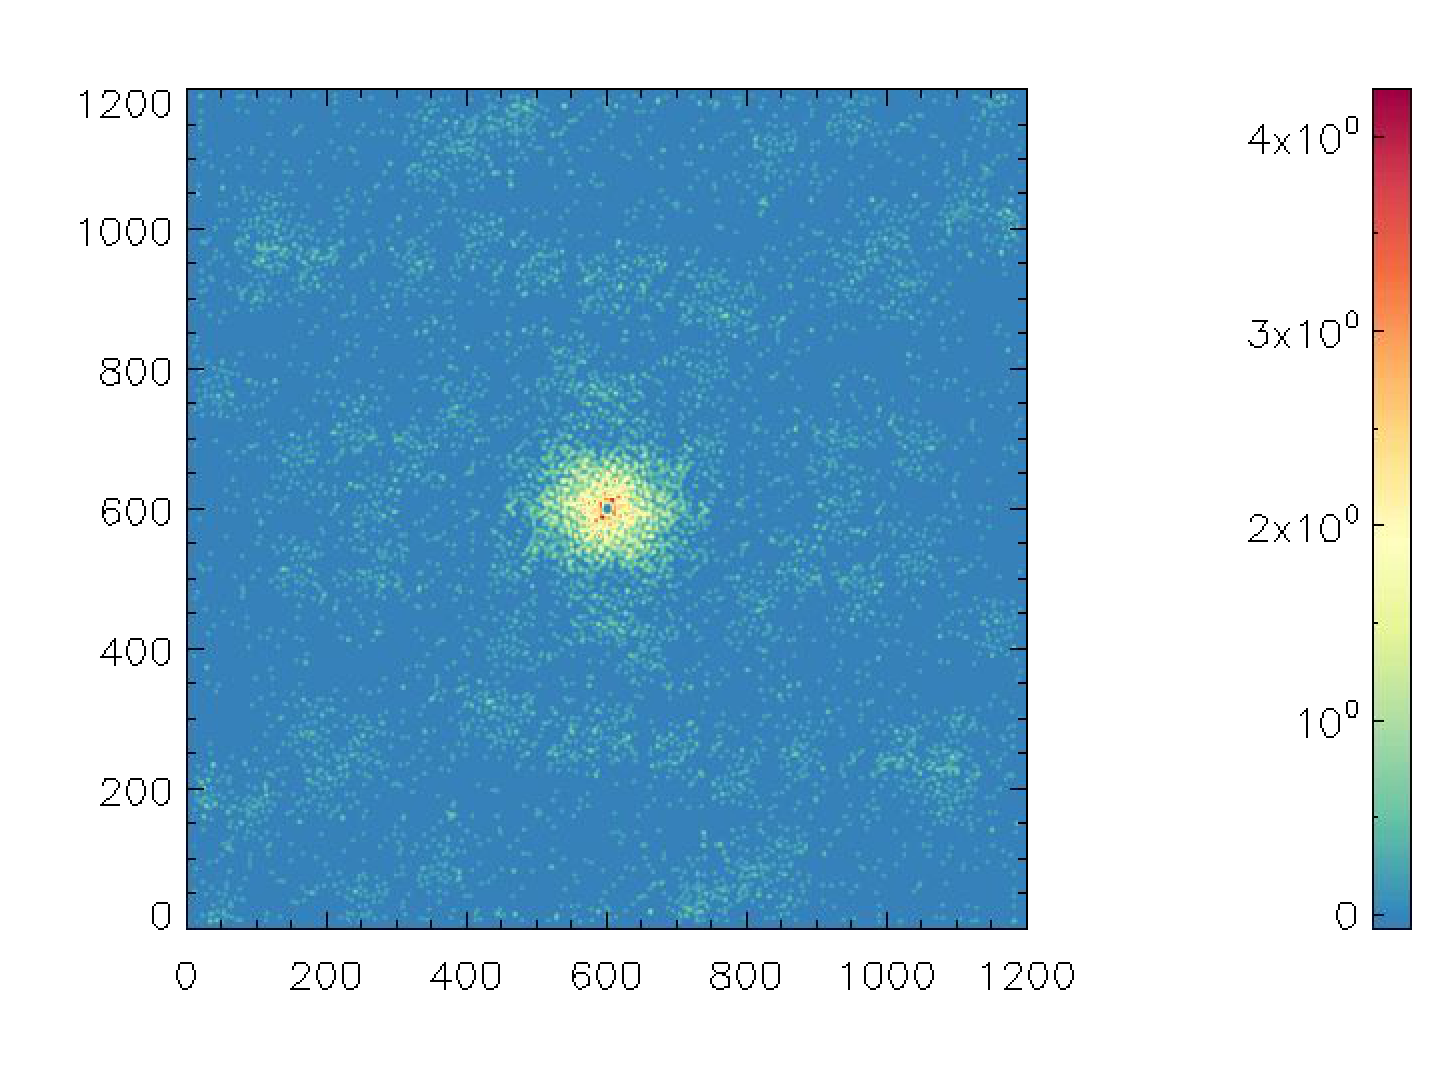
\includegraphics[scale=.2]{master run}
    \caption{A slice of the 0th frequency of a UVF weights cube with the interpolation grid as the observation's own orthoslant grid}
    \label{fig:mine}
\end{figure}

\begin{figure}[h!]
    \centering
    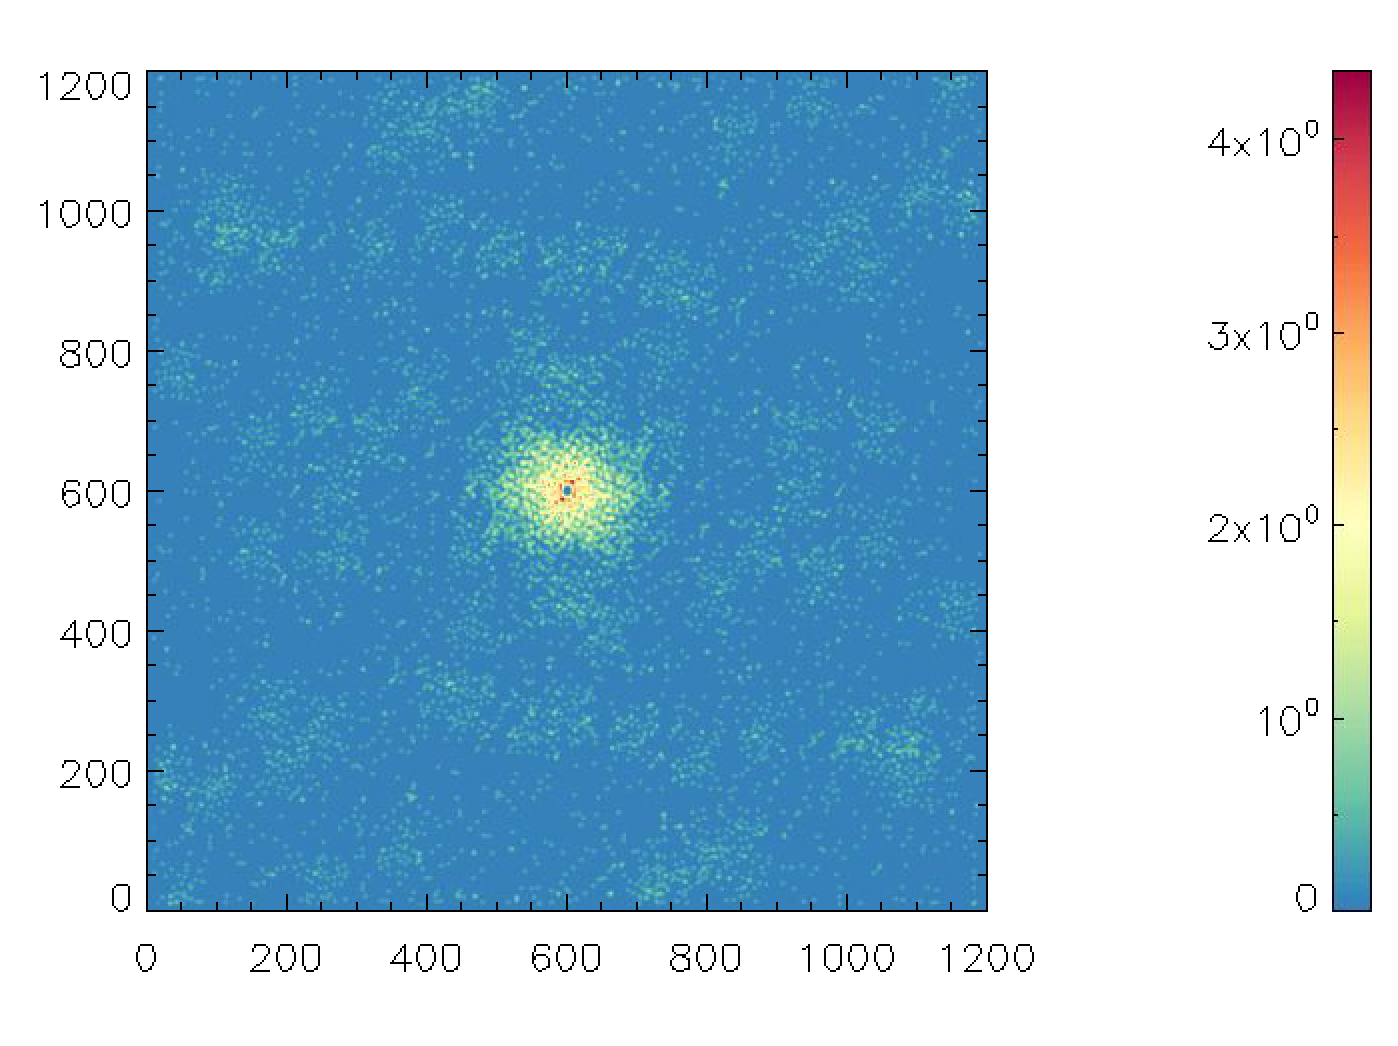
\includegraphics[scale=.2]{my run}
    \caption{A slice of the 0th frequency of a UVF weights cube with the original FHD code, no interpolation done}
    \label{fig:orig}
\end{figure}

\begin{figure}[h!]
    \centering
    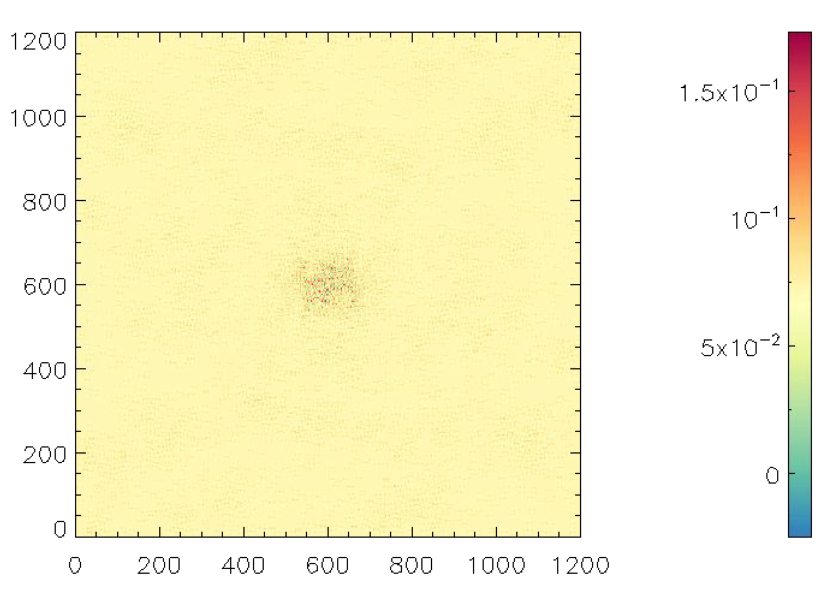
\includegraphics[scale=.7]{Screen Shot 2020-11-19 at 12.09.49 PM (1).png}
    \caption{Difference of a slice of the 0th frequency of a UVF weights cube.  No interpolation minus orthoslant interpolation.}
    \label{fig:diff}
\end{figure}

\section{Conclusion}
This memo covers the initial investigation into an aliasing systematic in the FHD/\eppsilon{} pipeline. The current recomendation to avoid this systematic is to limit the ps\_kspan keyword to 200 wavelengths when possible in analysis. Currently this cuts the sparsely covered portions of the UV plane (long baselines) and does not significantly impact power spectrum measurements. Long term investigation of this systematic will require will require rewriting of the interpolation code. 
The code for this project is contained in the interpolation\_test branch of the FHD github repository (https://github.com/EoRImaging/FHD/tree/interpolation$\_$test). 

\newpage


\end{document}